\chapter{UYGULAMA GÜVENLİĞİ VE DEVSECOPS}

\section*{Giriş}
Uygulama güvenliği ve DevSecOps, modern yazılım geliştirme süreçlerinde güvenliğin entegrasyonunu sağlayan kritik yaklaşımlardır. Bu bölümde güvenli yazılım geliştirme, kod analizi teknikleri ve DevSecOps uygulamalarını ele alacağız.

\section{Güvenli Yazılım Geliştirme Yaşam Döngüsü (SSDLC)}

Güvenli Yazılım Geliştirme Yaşam Döngüsü (SSDLC), yazılım geliştirme sürecinin her aşamasına güvenlik kontrollerinin ve uygulamalarının entegre edilmesini sağlayan bir metodolojidir. Geleneksel yazılım geliştirme modelleri, güvenliği genellikle son aşamada, yani test veya dağıtım aşamasında ele alırken, SSDLC bu yaklaşımın yetersiz olduğunu savunur. Güvenlik, geliştirme sürecinin başlangıcından itibaren bir öncelik olarak kabul edilmelidir. Bu proaktif yaklaşım, güvenlik açıklarının erken tespit edilmesini ve düzeltilmesini sağlayarak, hem maliyeti düşürür hem de genel yazılım kalitesini artırır.

\subsection{Güvenliğin Tasarımda Olması (Security by Design) ve Sola Kaydırma (Shift-Left) Güvenlik Yaklaşımları}

Güvenliğin tasarımda olması prensibi, güvenlik hususlarının bir sistemin temel mimarisine en başından itibaren dahil edilmesini öngörür. Bu yaklaşımın temel amacı, daha sonra tüm sistemi yeniden tasarlamayı gerektirecek ciddi tasarım kusurlarının oluşmasını önlemektir. Güvenlik, geliştirme sürecinin bir eklentisi veya son adımı olarak değil, projenin en temel yapı taşlarından biri olarak ele alınır.
Bu felsefeyi destekleyen anahtar metodoloji ise "Sola Kaydırma" (Shift-Left) güvenlik yaklaşımıdır. Sola kaydırma, güvenlik pratiklerinin geleneksel olarak geliştirme sürecinin son aşamalarına bırakılması yerine, planlama, tasarım ve kodlama gibi en erken safhalara taşınmasını ifade eder. Bu yaklaşımın temel amacı, güvenlik açıklarını üretime girmeden önce tespit edip düzeltmektir, çünkü bu, düzeltme maliyetini ve çabasını önemli ölçüde azaltır.
Sola kaydırma, sadece güvenlik araçlarının geliştirme boru hattına eklenmesiyle sınırlı değildir. Bu yaklaşımın başarısı, aynı zamanda derin bir kültürel dönüşümü gerektirir. Geleneksel "kodu duvardan atma" (toss it over the wall) modelinde, geliştiriciler kodu yazıp güvenlik ekibine teslim eder, güvenlik testleri ise ayrı bir silo içinde gerçekleştirilir. Bu durum, güvenlik testlerinin geliştirme hızını yavaşlatması ve son dakika sorunlarına yol açmasıyla sonuçlanabilir. Sola kaydırma ise geliştiricilerin güvenliği kendi sorumlulukları olarak benimsemesini, güvenlik uzmanlarının da bu süreci kolaylaştırıcı bir rol üstlenmesini gerektirir. Geliştiricilerin iş akışına entegre olan, soyut ve hızlı geri bildirim sağlayan araçlar ve politikalar, bu yaklaşımın benimsenmesini hızlandırır. Bu sayede, geliştiricilerin güvenlik farkındalığı artar ve daha güvenli kod yazma alışkanlıkları kazanılır, bu da genel olarak daha güvenli yazılımların ortaya çıkmasına yol açan bir döngü oluşturur.
Bu felsefenin etkileri, yalnızca uygulama katmanıyla sınırlı değildir. Bulut yerlisi (cloud-native) mimarilerin yaygınlaşmasıyla birlikte, altyapının da kod olarak (IaC) yönetilmesi mümkün hale gelmiştir. Bu durum, altyapı güvenliğinin de sola kaydırılabileceği yeni bir alan yaratmıştır. IaC taraması, hatalı yapılandırılmış ağ portları veya sabit kodlanmış kimlik bilgileri gibi riskleri, altyapı canlı bir ortamda saldırı yüzeyi oluşturmadan önce tespit etmeyi sağlar. Bu tür proaktif ve önleyici güvenlik kontrolleri, sistemin genel güvenlik duruşunu güçlendirir.

\subsection{Tehdit Modelleme Metodolojileri}

Tehdit modelleme, bir sistemdeki olası tehditleri, zafiyetleri ve açıklıkları sistematik olarak belirleme, listeleme ve önceliklendirme sürecidir. Bu süreç, yazılımın daha tasarlanma aşamasındayken proaktif olarak güvenlik önlemlerinin alınmasını sağlar. Farklı metodolojiler, tehditleri farklı açılardan ele alarak kuruluşların ihtiyaçlarına özel çözümler sunar.



\begin{itemize}
\item \textbf{STRIDE Metodolojisi:} Microsoft tarafından geliştirilen STRIDE, tehditleri altı temel kategoriye ayırarak bir çerçeve sunar:
\begin{itemize}
\item \textbf{S}poofing (Kimliğe Bürünme): Kimlik doğrulama kontrollerini hedef alır.
\item \textbf{T}ampering (Kurcalama): Veri bütünlüğünü tehlikeye atar.
\item \textbf{R}epudiation (Red): İzlenebilirlik ve loglama süreçlerini engellemeyi amaçlar.
\item \textbf{I}nformation Disclosure (Bilgi Açığa Çıkarma): Gizli bilgilerin ifşa edilmesini içerir.
\item \textbf{D}enial of Service (Hizmet Reddi): Erişilebilirliği engeller.
\item \textbf{E}levation of Privilege (Yetki Yükseltme): Yetkilendirme kontrollerini aşmayı amaçlar.
\end{itemize}

\begin{figure}[H]
    \centering
    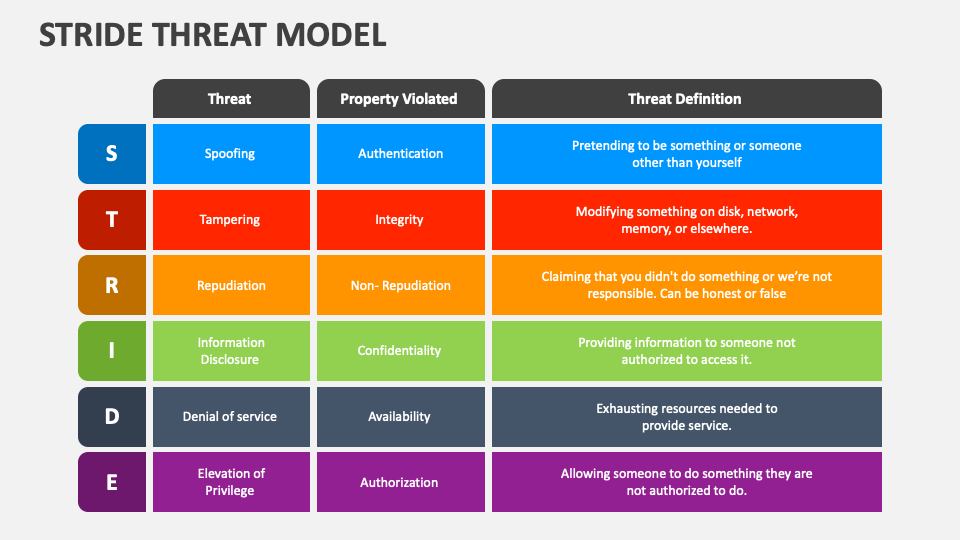
\includegraphics[width=0.7\textwidth]{img/stride-threat-model.png}
    \caption{Microsoft STRIDE Tehdit Modelleme Çerçevesi}
    \label{fig:stride-threat-model}
\end{figure}

STRIDE, genellikle geliştirme sürecinin tasarım aşamasında kullanılır ve sistem mimarisini analiz ederek potansiyel tehdit kategorilerini belirlemeye yardımcı olur.
\item \textbf{DREAD Metodolojisi:} DREAD, bir tehdidin ciddiyetini değerlendirmek için kullanılan nicel bir modeldir. Genellikle STRIDE ile birlikte kullanılır; STRIDE tehditleri belirlerken, DREAD bunların önceliklendirilmesine yardımcı olur. Her bir tehdit, beş kritere göre 1'den 10'a kadar bir puanla derecelendirilir:
\begin{itemize}
    \item \textbf{D}amage (Hasar): Saldırının potansiyel etkisi.
    \item \textbf{R}eproducibility (Tekrarlanabilirlik): Saldırının ne kadar kolay tekrarlanabildiği.
    \item \textbf{E}xploitability (İstismar Edilebilirlik): Zafiyetin ne kadar kolay istismar edilebildiği.
    \item \textbf{A}ffected Users (Etkilenen Kullanıcılar): Etkilenen kullanıcı sayısı.
    \item \textbf{D}iscoverability (Keşfedilebilirlik): Zafiyetin ne kadar kolay keşfedilebildiği.
\end{itemize}
Bu puanların ortalaması alınarak her bir tehdide bir önem derecesi atanır ve böylece düzeltme stratejileri önceliklendirilir.
\item \textbf{PASTA Metodolojisi (Process for Attack Simulation and Threat Analysis):} PASTA, yedi adımlı, saldırgan odaklı ve risk merkezli kapsamlı bir metodolojidir. Bu yaklaşım, tehditleri iş hedefleriyle ilişkilendirerek olgun güvenlik programlarına sahip büyük kuruluşlar için idealdir.
\end{itemize}
Tehdit modelleme çerçeveleri birbirini dışlayan yaklaşımlar değildir, aksine birbirini tamamlayan araçlar olarak kullanılabilir. STRIDE gibi bir model, potansiyel tehditlerin varlığını sistematik bir şekilde ortaya çıkarırken, DREAD bu tehditlerin ne kadar acil bir risk oluşturduğunu belirlemek için kullanılır. Bu sinerjik kullanım, sınırlı kaynakların en kritik güvenlik sorunlarına yönlendirilmesini sağlar. Ayrıca, PASTA'nın iş süreçlerini ve teknik tehditleri bir araya getirme yaklaşımı, tehdit modellemenin sadece teknik bir egzersiz değil, aynı zamanda stratejik bir iş faaliyeti olduğunu gösterir.
\textbf{Uygulamalı Senaryo:}
Bir e-ticaret uygulamasının kullanıcı profili güncelleme bileşenine yönelik tehdit modellemesi şu adımlarla gerçekleştirilebilir:
\begin{itemize}
\item Veri Akış Şeması (DFD) oluşturularak, kullanıcının profiline ilişkin verilerin nasıl hareket ettiği görselleştirilir.
\item STRIDE kullanılarak, her bir veri akışı ve işlem için olası tehditler listelenir. Örneğin, \texttt{HTTP POST} isteğiyle gönderilen kullanıcı verileri için "Kurcalama" tehdidi incelenir.
\item Tespit edilen her tehdit, DREAD kriterlerine göre puanlanarak en yüksek riske sahip olanlar önceliklendirilir. Bu sayede, güvenlik ekipleri en acil sorunlara odaklanabilir.
\end{itemize}
\subsection{Güvenli Kodlama Standartları ve En İyi Uygulamalar}
Güvenli kodlama, zafiyetlerin kaynak kod seviyesinde oluşmasını engellemek için benimsenen bir dizi disiplinli yaklaşımdır. Uygulamaların güvenliğini temelden sağlamlaştırmak için belirli prensiplere uyulması gerekir.
\begin{itemize}
\item \textbf{Varsayılan Olarak Reddetme (Default Deny):} Erişim kararlarının, özellikle yetkilendirme ve erişim kontrollerinde, varsayılan olarak reddetme üzerine inşa edilmesi esastır. Bu, yalnızca açıkça izin verilen koşullar altında erişime izin verilmesini sağlar.
\item \textbf{En Az Yetkilendirme (Principle of Least Privilege):} Her süreç veya kullanıcı, görevini tamamlamak için gerekli olan en az yetki setiyle çalışmalıdır. Bu yaklaşım, bir saldırganın sistemde yetki yükseltme yapma olasılığını azaltır.
\item \textbf{Girdi Doğrulama:} Tüm güvenilmeyen veri kaynaklarından (kullanıcı girdisi, API yanıtları, çevre değişkenleri) gelen verilerin titizlikle doğrulanması, zafiyetlerin büyük bir kısmını önleyebilir.
\item \textbf{Merkezi Güvenlik Kontrolleri:} Kimlik doğrulama, yetkilendirme ve girdi doğrulama gibi güvenlik işlevlerinin, tüm uygulama genelinde tek ve merkezi bir rutin aracılığıyla yapılması tavsiye edilir. Bu, güvenlik politikalarının tutarlı bir şekilde uygulanmasını sağlar.
\item \textbf{Savunmada Derinlik (Defense in Depth):} Bir savunma katmanının başarısız olması durumunda diğerlerinin koruma sağlaması için çoklu savunma stratejilerinin uygulanması gerekir. Bu prensip, güvenli programlama tekniklerinin güvenli çalışma zamanı ortamlarıyla birleştirilmesi gibi yöntemlerle desteklenebilir.
\end{itemize}
\subsection{Güvenlik Kod İncelemesi ve Statik Analiz (SAST) Entegrasyonu}
Statik Uygulama Güvenlik Testi (SAST), uygulamanın kaynak kodunu, bayt kodunu veya ikili kodunu çalıştırmadan analiz eden bir "beyaz kutu" test metodolojisidir. SAST, geliştirme yaşam döngüsünün en erken aşamalarında zafiyetleri (örn. SQL enjeksiyonları, arabellek taşmaları) tespit etme yeteneğine sahiptir.
Bir SAST aracı, kodu ayrıştırarak soyut bir sözdizimi ağacı (AST) oluşturur. Bu ağaç, kodun yapısını temsil eder ve aracın veri akışını izlemesine olanak tanır. Analiz, OWASP Top 10 ve CWE/SANS Top 25 gibi bilinen güvenlik standartlarına ve kurallarına göre yapılır. SAST, entegre geliştirme ortamlarına (IDE), versiyon kontrol sistemlerine ve CI/CD hatlarına entegre edilebilir. Bu sayede geliştiriciler, kodlarını kaydederken veya birleştirme isteği (pull request) oluştururken anında geri bildirim alabilirler. SAST'ın en büyük zorluklarından biri, yanlış pozitif (false positives) uyarı sayısının yüksek olabilmesidir. Ayrıca, SAST araçları kodda temsil edilmeyen, örneğin sunucu yapılandırması gibi sorunları tespit edemez.
\subsection{CI/CD Pipeline'larında Güvenlik Testi Entegrasyonu}
Modern yazılım geliştirme süreçlerinde, güvenlik testleri CI/CD (Sürekli Entegrasyon/Sürekli Dağıtım) boru hatlarına entegre edilerek otomatize edilir ve sürekli hale getirilir.
\begin{itemize}
\item \textbf{SAST:} SAST, CI/CD boru hattına \texttt{pre-commit} hook'ları veya build aşaması gibi en erken noktalarda entegre edilir. Örneğin, bir geliştirici kodunu göndermeden önce yerel bir tarama yaparak basit hataları hızlıca düzeltebilir.
\item \textbf{DAST (Dynamic Application Security Testing):} DAST, çalışan bir uygulama üzerinde "siyah kutu" testi yaparak gerçek bir saldırıyı simüle eder. Bu, SAST'ın gözden kaçırabileceği iş mantığı hataları, kimlik doğrulama bypass'ları veya yapılandırma zafiyetleri gibi çalışma zamanı (runtime) sorunlarını ortaya çıkarır. DAST taramaları genellikle boru hattının sonlarına doğru, staging veya QA ortamında otomatik olarak çalıştırılır.
\item \textbf{IAST (Interactive Application Security Testing):} IAST, SAST ve DAST'ın hibrit birleşimidir. Uygulama çalışırken içeriden analiz yaparak, zafiyetin tam olarak hangi kod satırında olduğunu saptar ve düşük yanlış pozitif oranıyla sonuç üretir. IAST, CI/CD hatlarına sorunsuz entegre olabilen tek dinamik test tekniği olarak öne çıkar ve geliştiricilere hızlı ve bağlamsal geri bildirim sağlar.
\end{itemize}
\textbf{Tablo 4.1.5a: AST Metodolojileri - Temel Özellikler}

\begin{tabular}{|p{2cm}|p{5cm}|p{3cm}|p{3cm}|}
\hline
\textbf{Metodoloji} & \textbf{Tanım} & \textbf{SDLC Konumu} & \textbf{Yöntem} \\
\hline
\textbf{SAST} & Statik Uygulama Güvenlik Testi & Plan, Kod, Build & Beyaz Kutu, Kod Analizi \\
\hline
\textbf{DAST} & Dinamik Uygulama Güvenlik Testi & Test, Dağıtım & Siyah Kutu, Uygulama Simülasyonu \\
\hline
\textbf{IAST} & Etkileşimli Uygulama Güvenlik Testi & Test, QA & Hibrit (Beyaz + Siyah Kutu) \\
\hline
\textbf{RASP} & Çalışma Zamanı Uygulama Koruması & Çalışma (Runtime) & Uygulama İçi İzleme \\
\hline
\textbf{SCA} & Yazılım Bileşen Analizi & Plan, Kod, Build & Bağımlılık Taraması \\
\hline
\end{tabular}

\textbf{Tablo 4.1.5b: AST Metodolojileri - Kapsamlar ve Özellikler}

\begin{tabular}{|p{2cm}|p{4cm}|p{4cm}|p{3.5cm}|}
\hline
\textbf{Metodoloji} & \textbf{Kapsadığı Zafiyetler} & \textbf{Avantajları} & \textbf{Zorlukları} \\
\hline
\textbf{SAST} & SQLi, XSS, Buffer Overflow, Hardcoded Secrets & Erken geri bildirim, geniş kapsam & Yüksek yanlış pozitif \\
\hline
\textbf{DAST} & SQLi, XSS, Kimlik Doğrulama, İş Mantığı & Gerçek saldırı simülasyonu & Kaynak kodu bilmez \\
\hline
\textbf{IAST} & SQLi, XSS, Veri Akışı Zafiyetleri & Düşük yanlış pozitif & Karmaşık kurulum \\
\hline
\textbf{RASP} & Bilinen ve sıfır-gün saldırıları & Gerçek zamanlı koruma & Performans etkisi \\
\hline
\textbf{SCA} & Kütüphane zafiyetleri, lisans uyumu & Açık kaynak risk yönetimi & Sadece bilinen zafiyetler \\
\hline
\end{tabular}

\section{Web Uygulama Güvenliği ve OWASP Çerçevesi}

Web uygulama güvenliği, modern siber güvenlik stratejilerinin temel taşlarından biridir. Open Web Application Security Project (OWASP), web uygulamalarının güvenliğini artırmak için standartlar, araçlar ve en iyi uygulamalar sunan, kar amacı gütmeyen bir kuruluştur. OWASP'ın kaynak havuzu şunları içerir:

\begin{itemize}
\item \textbf{OWASP Top 10:} Web uygulamalarına yönelik en kritik on güvenlik riskini sıralayan ve düzenli olarak güncellenen bir liste. Bu liste, geliştiricilerin ve güvenlik profesyonellerinin en yaygın saldırı vektörlerine karşı savunma stratejileri oluşturmasına yardımcı olur.

\item \textbf{OWASP Testing Guide:} Kapsamlı bir web uygulama güvenlik testi rehberi. Test süreçlerini, metodolojileri ve araçları detaylıca açıklar.

\item \textbf{OWASP Code Review Guide:} Güvenli kod inceleme pratikleri için yol gösterici bir kaynak. Geliştiricilere ve güvenlik uzmanlarına yönelik rehberlik sağlar.

\item \textbf{OWASP Software Assurance Maturity Model (SAMM):} Organizasyonların yazılım güvenliği programlarını değerlendirmeleri ve geliştirmeleri için bir çerçeve sunar.

\item \textbf{OWASP Security Knowledge Framework (SKF):} Güvenli yazılım geliştirme için bir eğitim platformu ve kılavuz.

\item \textbf{OWASP DevSecOps Maturity Model:} DevSecOps olgunluğunu değerlendirmek ve geliştirmek için bir çerçeve sunar.

\item \textbf{OWASP Mobile Security Testing Guide (MASTG):} Mobil uygulama güvenlik testi için kapsamlı bir rehber.

\item \textbf{OWASP Web Security Testing Guide (WSTG):} Web uygulaması güvenlik testi için metodolojiler ve örnekler sunar.

\item \textbf{OWASP API Security Top 10:} API güvenliğindeki en kritik riskleri tanımlar.
\end{itemize}

OWASP, düzenli olarak güncellenen, gönüllü topluluğun katkılarıyla gelişen ve açık kaynak prensiplerini benimseyen bir projedir. Kuruluşların güvenlik olgunluğunu artırmak için birçok farklı araç ve çerçeve sunar.

\subsection{OWASP Top 10 Güvenlik Açıkları ve Azaltma Stratejileri}

OWASP Top 10, web uygulamaları için en kritik on riskin konsensüs listesidir. Bu liste, güvenlik uzmanlarının ve geliştiricilerin en önemli zafiyetlere odaklanmasına yardımcı olur.

\begin{figure}[H]
    \centering
    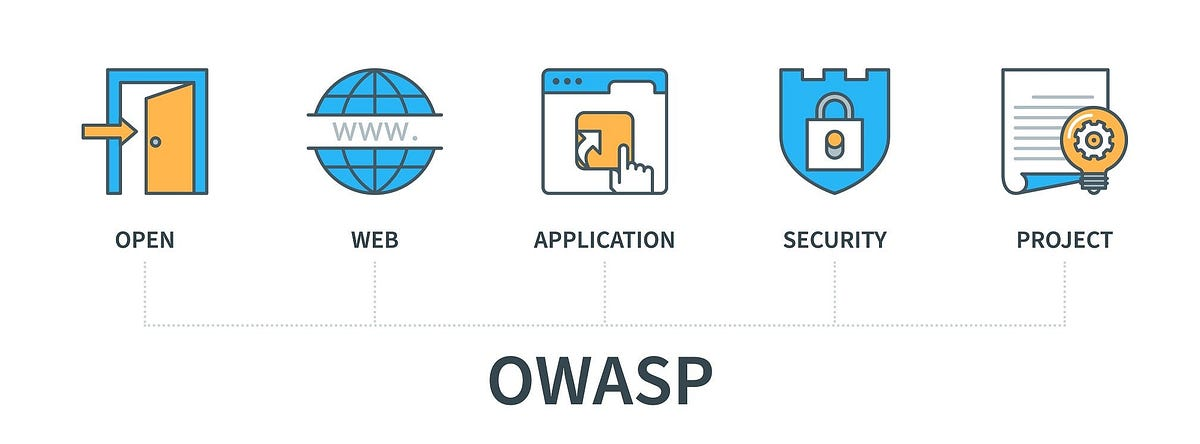
\includegraphics[width=0.6\textwidth]{img/owasp-standsfor.png}
    \caption{OWASP (Open Web Application Security Project) Logosu ve Açılımı}
    \label{fig:owasp-logo}
\end{figure}



\begin{itemize}
\item \textbf{A01:2021 Bozuk Erişim Kontrolü (Broken Access Control):} 2021 listesinde birinci sıraya yükselen bu zafiyet, bir saldırganın yetkisi olmayan kullanıcı hesaplarına veya işlevlere erişimini sağlar. Örneğin, bir URL'deki kullanıcı kimliğini temsil eden birincil anahtarın değiştirilmesiyle, bir saldırgan başka bir kullanıcının hesabını görüntüleyebilir veya düzenleyebilir. Bu tür zafiyetlerin giderilmesi için IAST araçları kullanılabilir ve mimari tasarımda güven sınırları oluşturulması gerekebilir.
\item \textbf{A02:2021 Kriptografik Başarısızlıklar (Cryptographic Failures):} Daha önce "Hassas Veri Açığa Çıkması" olarak bilinen bu risk, parolalar, kimlik numaraları gibi hassas verilerin depolanması veya iletilmesi sırasında yetersiz şekilde korunmasıyla ilgilidir. Zayıf şifreleme algoritmaları veya sabit kodlanmış kriptografik anahtarlar gibi kök nedenlere odaklanır. SAST ve SCA araçları, zayıf şifreleme gücü ve riskli algoritmaları tarayarak bu riskleri azaltmaya yardımcı olurken, IAST sürekli izleme sağlar.
\item \textbf{A03:2021 Enjeksiyon (Injection):} Listede üçüncü sırada yer alan enjeksiyon, güvensiz verilerin komut veya sorgu olarak yorumlanması sonucu meydana gelir. En yaygın türleri SQL enjeksiyonu ve artık bu kategoriye dahil edilen XSS'tir.
\end{itemize}

\subsection{Girdi Doğrulama, Çıktı Kodlama ve Parametreli Sorgular}

Bu üç teknik, enjeksiyon saldırılarına karşı birincil savunma mekanizmalarıdır.

\begin{itemize}
\item \textbf{Girdi Doğrulama (Input Validation):} Güvenilmeyen kaynaklardan gelen verinin, beklenen format, tip ve uzunluk gibi önceden tanımlanmış kriterlere uyduğunu doğrular. En güvenli yaklaşım, yalnızca kabul edilebilir karakter veya formatları tanımlayan bir "beyaz liste" (allowlist) kullanmaktır, "kara liste" (denylist) ise eksik olabilir ve yeni saldırı vektörlerine karşı savunmasız kalabilir. Sunucu tarafında uygulanması zorunludur, çünkü istemci tarafı doğrulama kolayca atlatılabilir.
\item \textbf{Çıktı Kodlama (Output Encoding):} Bir uygulamanın, kullanıcıdan gelen veriyi tarayıcı veya başka bir yorumlayıcıya göndermeden önce potansiyel olarak zararlı karakterleri güvenli bir formata dönüştürmesidir. Bu, karakterlerin kod olarak değil, salt metin olarak görüntülenmesini sağlar ve XSS saldırılarını önlemede kritik bir rol oynar.
\item \textbf{Parametreli Sorgular (Parameterized Queries):} SQL enjeksiyonuna karşı en etkili savunma yöntemidir. Bu teknik, SQL kod yapısını kullanıcıdan gelen veriden ayırır, böylece girdi yalnızca bir veri değeri olarak işlenir ve kötü amaçlı komutların veritabanı tarafından yürütülmesini engeller.
\end{itemize}

\subsection{Kimlik Doğrulama ve Oturum Yönetimi Güvenliği}

Kimlik doğrulama, kullanıcıyı doğrulamayı, oturum yönetimi ise bu doğrulama sonrası kullanıcı oturumunu güvenli bir şekilde sürdürmeyi amaçlar.

\begin{itemize}
\item \textbf{Oturum Güvenlik Açıkları:} İlgili riskler arasında bir saldırganın geçerli bir oturum belirtecini ele geçirdiği \textbf{Oturum Korsanlığı (Session Hijacking)} ve bir kullanıcıyı önceden belirlenmiş bir oturum kimliği kullanmaya zorladığı \textbf{Oturum Sabitleme (Session Fixation)} yer alır.
\item \textbf{En İyi Uygulamalar:} Oturum kimlikleri, yeterli rastgeleliğe (en az 64 bit entropi) sahip bir CSPRNG (Kriptografik Olarak Güvenli Sözde Rastgele Sayı Üreteci) ile oluşturulmalıdır. Oturum çerezlerinin \texttt{HttpOnly} bayrağı ile korunması, JavaScript'in çereze erişimini engeller ve XSS saldırılarına karşı bir savunma katmanı sağlar. Oturumların, hem kullanıcı çıkış yaptığında hem de bir süre işlem yapılmadığında güvenli bir şekilde sonlandırılması gereklidir.
\end{itemize}

\subsection{Cross-Site Scripting (XSS) ve Cross-Site Request Forgery (CSRF)}

XSS ve CSRF, web uygulamalarının kullanıcılarına duyduğu "güven"i istismar eden iki farklı ancak birbiriyle ilişkili saldırı türüdür.

\begin{itemize}
\item \textbf{XSS (Siteler Arası Komut Dosyası Çalıştırma):} Saldırgan, bir web uygulamasına kötü amaçlı bir komut dosyası enjekte ederek bu betiğin diğer kullanıcıların tarayıcılarında çalışmasını sağlar. Bu, uygulamanın kullanıcı girdisini yeterince filtrelememesinden kaynaklanır. Azaltım stratejileri, girdi doğrulaması, çıktı kodlaması ve DOMPurify gibi kütüphanelerle HTML sanitizasyonunu içerir.
\item \textbf{CSRF (Siteler Arası İstek Sahteciliği):} Bu saldırıda, bir saldırgan bir kullanıcıyı, rızası olmadan bir eylem gerçekleştirmesi için sahte bir istek göndermesi için kandırır. Saldırganın hedefi, uygulamanın kullanıcının oturum kimliğine ve dolayısıyla isteğin meşruiyetine olan güvenini istismar etmektir. En yaygın savunma, her istek için benzersiz ve öngörülemez bir \textbf{CSRF belirteci} (token) kullanmaktır.
\end{itemize}

XSS ve CSRF, farklı güvenlik zafiyetleri olmasına rağmen, birbirlerinin savunmasını etkileyebilir. Bir saldırgan XSS ile başarılı olursa, \texttt{HttpOnly} bayrağı olmayan oturum çerezlerini ele geçirerek oturum korsanlığına zemin hazırlayabilir. Ancak, CSRF belirteçleri gibi bir kontrol, XSS saldırılarına karşı ikincil bir savunma katmanı sağlayabilir. Bir saldırgan XSS ile kötü amaçlı bir betik enjekte etse bile, bu betik, istek için geçerli olan benzersiz CSRF belirtecine erişemez ve bu da saldırının engellenmesine yardımcı olur. Bu durum, güvenlik kontrollerinin birbirini desteklemesi gerektiğini vurgulayan "savunmada derinlik" prensibinin bir yansımasıdır.

\subsection{İçerik Güvenlik Politikası (CSP) ve Güvenlik Başlıkları}

İçerik Güvenlik Politikası (CSP), bir web uygulamasının güvenlik modeline ikinci bir savunma katmanı ekleyen bir güvenlik başlığıdır. Sunucu tarafından gönderilen bu HTTP başlığı, tarayıcıya, betikler, stiller, resimler gibi hangi kaynaklardan içerik yükleyebileceğini bildirir.

CSP, XSS saldırılarına karşı birden fazla şekilde koruma sağlar:

\begin{itemize}
\item \textbf{Satır İçi Betik Kısıtlaması:} \texttt{inline} (satır içi) \textless script\textgreater{} etiketlerinin çalışmasını engeller.
\item \textbf{Uzak Kaynak Kısıtlaması:} Rastgele sunuculardan betik yüklenmesini engeller.
\item \textbf{Güvenli Olmayan Fonksiyonların Engellenmesi:} \texttt{eval()} gibi güvensiz JavaScript fonksiyonlarının yürütülmesini kısıtlar.
\item \textbf{Form Kısıtlaması:} HTML formlarının yalnızca belirlenen güvenilir hedeflere veri göndermesini sağlar, bu da kimlik avı formlarının enjekte edilmesini önler.
\end{itemize}

CSP, "yalnızca raporlama" moduyla test edilebilir veya doğrudan etkinleştirilerek zorunlu hale getirilebilir. Güvenlik başlıklarının doğru bir şekilde yapılandırılması, uygulamanın genel güvenlik duruşunu önemli ölçüde artırır.

\section{API Güvenliği ve Microservices Mimarisi}

API'ler (Application Programming Interfaces), modern yazılım mimarilerinin temel bir bileşenidir ve farklı uygulamaların birbirleriyle iletişim kurmasını sağlar. Mikroservis mimarileri, büyük ve monolitik uygulamaları daha küçük, bağımsız hizmetlere ayırarak geliştirme ve dağıtım süreçlerini kolaylaştırır. Ancak, bu mimari aynı zamanda yeni güvenlik zorlukları da ortaya çıkarır. Her bir mikroservis ve API, potansiyel bir saldırı yüzeyi oluşturur ve bu nedenle güvenli bir şekilde tasarlanmalı ve yönetilmelidir.

\subsection{RESTful API Güvenliği En İyi Uygulamaları}

RESTful API'ler, web uygulamalarıyla aynı seviyede veya daha fazla güvenlik riskine sahiptir. Bu nedenle, tasarım aşamasından itibaren katı güvenlik prensiplerinin uygulanması gereklidir.

\begin{itemize}
\item \textbf{Her Zaman TLS Şifrelemesi Kullanın:} Tüm API iletişimleri, uçtan uca veri şifrelemesi sağlamak için TLS (Transport Layer Security) ile korunmalıdır. Bu, ağ trafiği içindeki parolalar, API anahtarları veya tokenlar gibi hassas bilgilerin gizliliğini sağlar.
\item \textbf{Güçlü Kimlik Doğrulama ve Yetkilendirme Modeli:} API anahtarları ve güvenlik tokenları gibi yöntemlerle ölçeklenebilir bir modelin uygulanması esastır. Bu süreç, özellikle OAuth 2.0 ve OpenID Connect gibi standartlarla entegre bir şekilde yürütüldüğünde, daha güvenli ve yönetilebilir hale gelir.
\item \textbf{Hassas Bilgileri URL'de Tutmayın:} Bir RESTful API tasarım hatası, kullanıcı kimlik bilgileri veya tokenlar gibi hassas verilerin URL'lere eklenmesidir. Bu, TLS kullanılsa dahi, verilerin sunucu günlüklerinde veya ağ cihazlarında kolayca keşfedilmesine yol açabilir.
\item \textbf{İstek ve Yanıtları Dar Tanımlayın:} Saldırganların API'leri kötü niyetli veya amaç dışı kullanmaya çalışacağını varsaymak önemlidir. Bu nedenle, gelen parametrelerin formatı, uzunluğu ve tipi gibi nitelikleri titizlikle doğrulanmalı, API yanıtları ise yalnızca açıkça izin verilen içerikle sınırlı tutulmalıdır.
\item \textbf{Sürekli API Keşfi:} "Gölge" (shadow) API'leri (standart süreçler dışında geliştirilenler) ve "zombi" (zombie) API'leri (unutulmuş eski altyapılardaki riskler) gibi varlıkları belirlemek için sürekli bir envanter yönetimi ve keşif yeteneği uygulanmalıdır.
\end{itemize}

\subsection{OAuth 2.0, OpenID Connect ve JWT Token Güvenliği}

Bu üç teknoloji, API güvenliği için modern kimlik doğrulama ve yetkilendirme standartlarını oluşturur.

\begin{itemize}
\item \textbf{OAuth 2.0:} Bir yetkilendirme çerçevesidir. Kullanıcının parolalarını paylaşmadan, bir uygulamaya kendi adına belirli kaynaklara erişim izni vermesini sağlar.
\item \textbf{OpenID Connect (OIDC):} OAuth 2.0 üzerine inşa edilmiş, kimlik doğrulama katmanı ekleyen bir protokoldür. Bir kullanıcının kimliğini doğrulamak ve temel profil bilgilerini almak için kullanılır.
\item \textbf{JWT (JSON Web Token):} JSON tabanlı, sıkıştırılmış ve güvenli bir belirteç formatıdır. OIDC ve OAuth 2.0'da kimlik ve erişim belirteçlerini iletmek için kullanılır.
\item \textbf{JWT Güvenliği:}
\begin{itemize}
\item \textbf{Doğrulama:} Gelen her JWT, her istekte imzası, süresi (\texttt{exp}) ve yayıncısı (\texttt{iss}) gibi iddialarının (\texttt{claims}) doğrulanması zorunludur. Bu, tokenın sahte veya kurcalanmış olmadığını garanti eder.
\item \textbf{Güvenli Saklama:} JWT'ler, Çapraz Site Komut Dosyası Çalıştırma (XSS) saldırılarına karşı \texttt{HttpOnly} ve \texttt{Secure} bayraklarına sahip çerezlerde saklanmalıdır. \texttt{localStorage} veya \texttt{sessionStorage} gibi tarayıcı depolama alanları, JavaScript tarafından erişilebilir oldukları için XSS'e karşı savunmasızdır.
\item \textbf{Kısa Yaşam Süresi:} JWT'lerin kısa ömürlü olması, token çalınması durumunda saldırganın etki süresini sınırlar. Bu tokenlar, daha uzun ömürlü ancak daha güvenli bir şekilde saklanan yenileme belirteçleriyle (refresh tokens) birlikte kullanılmalıdır.
\end{itemize}
\end{itemize}

\subsection{API Gateway Güvenlik Özellikleri ve Hız Sınırlandırma (Rate Limiting)}

Mikroservis mimarisinde, bir API Gateway, hizmetler için tek bir giriş noktası görevi görür. Bu merkezi konum, kimlik doğrulama, yetkilendirme, izleme ve özellikle hız sınırlama gibi güvenlik kontrollerinin tutarlı bir şekilde uygulanmasını sağlar.

\begin{itemize}
\item \textbf{Hız Sınırlandırma (Rate Limiting):} Bir istemcinin belirli bir zaman diliminde API'ye gönderebileceği istek sayısını kontrol eden bir mekanizmadır. Bu, hizmet reddi (DoS) ve kaba kuvvet saldırılarını önlemenin yanı sıra, sistemin aşırı yüklenmesini engeller ve adil kaynak dağılımını sağlar.
\item \textbf{Algoritmalar:} En yaygın kullanılan hız sınırlama algoritmaları arasında \textbf{Sabit Pencere Sayacı (Fixed Window Counter)}, \textbf{Kaydırılan Günlük (Sliding Log)} ve ani trafik artışlarını yönetmek için ideal olan \textbf{Token Kovası (Token Bucket)} yer alır.
\end{itemize}

\subsection{GraphQL Güvenlik Hususları}

GraphQL, esnekliği sayesinde geliştiriciler arasında popülerlik kazanmıştır, ancak bu esneklik kendine özgü güvenlik tehditlerini de beraberinde getirir.

\begin{itemize}
\item \textbf{DoS Saldırıları:} GraphQL'in iç içe geçmiş sorgulara (nested queries) izin vermesi, bir saldırganın tek bir istekte çok fazla kaynak talep ederek hizmet reddi (DoS) saldırısı gerçekleştirmesine olanak tanır.
\item \textbf{Azaltım:} Sorgu derinliği ve maliyet analizi sınırlamaları uygulanmalıdır. Bu kontroller, bir sorgunun karmaşıklığına göre sunucunun tüketebileceği maksimum kaynak miktarını sınırlar.
\item \textbf{Yetkilendirme:} GraphQL API'leri, talep edilen veriler üzerinde yetkilendirme kontrollerini titizlikle uygulamalıdır. Yetkilendirme kontrollerinin hem düğümler (\texttt{nodes}) hem de kenarlar (\texttt{edges}) üzerinde uygulanması, Broken Object Level Authorization (BOLA) gibi zafiyetleri önler.
\item \textbf{Güvenli Yapılandırma:} Üretim ortamlarında, API'nin yapısını keşfetmeyi sağlayan \textbf{Introspection} sorguları devre dışı bırakılmalı veya yalnızca yetkili kullanıcılara açık olmalıdır. Ayrıca, hata mesajlarında gereksiz iç sistem bilgilerinin (örn. yığın izleri) açığa çıkması engellenmelidir.
\end{itemize}

\subsection{Microservices İletişim Güvenliği (mTLS, Service Mesh)}

Mikroservisler arası iletişim, genellikle bir ağ üzerinden gerçekleştiği için ortadaki adam (MITM) ve kimliğe bürünme saldırılarına açıktır.

\begin{itemize}
\item \textbf{mTLS (Mutual TLS):} Geleneksel TLS'nin aksine, mTLS'de hem istemci hem de sunucu, iletişim başlamadan önce birbirlerinin kimliklerini doğrular. Bu, sıfır güven (zero-trust) mimarilerinin temelini oluşturan, karşılıklı kimlik doğrulama ve şifreleme sağlar. Uygulama, OpenSSL gibi araçlarla sertifika ve anahtar çiftleri oluşturularak adım adım uygulanabilir.
\item \textbf{Service Mesh:} Mikroservisler arası iletişimin güvenliğini, izlenebilirliğini ve yönetimini sağlayan bir altyapı katmanıdır. Service Mesh, mTLS'i hizmetler için otomatik olarak yönetir, bu da her bir hizmetin kendi güvenlik mantığını uygulamasına gerek kalmamasını sağlar.
\end{itemize}

Service Mesh, mTLS'in tek başına yeterli olmadığı yetkilendirme sorununu da ele alır. mTLS bir hizmetin kimliğini doğrular, ancak o hizmetin belirli bir eylemi yapmaya yetkili olup olmadığını garantilemez. Service Mesh, yetkilendirme kurallarını merkezi olarak tanımlama ve uygulama yeteneği sunarak, sıfır güven mimarisinin "asla güvenme, her zaman doğrula" prensibini en iyi şekilde uygulamayı mümkün kılar. Bu, güvenlik politikasını ağ katmanından daha granüler olan iş yükü (pod) seviyesine taşıyarak daha sağlam bir koruma sağlar.

\section{Uygulama Güvenlik Testi (AST) Metodolojileri}

Uygulama Güvenlik Testi (AST), yazılım geliştirme yaşam döngüsü boyunca güvenlik açıklarını tespit etmek ve düzeltmek için kullanılan bir dizi metodolojiyi ifade eder. AST, statik, dinamik ve interaktif test yaklaşımlarını içerir.

\subsection{Statik Uygulama Güvenlik Testi (SAST) Araçları}

SAST, kaynak kodun, bayt kodun veya ikili kodun çalıştırılmadan analizini yapar. Bu "beyaz kutu" test metodolojisi, SQL enjeksiyonları, arabellek taşmaları ve XSS gibi güvenlik açıklarını, yazılım geliştirme yaşam döngüsünün çok erken aşamalarında, hatta kod derlenmeden önce bile tespit edebilir. SAST araçları, kodun tamamını tarayarak potansiyel güvenlik zafiyetlerini belirler. Bu araçlar, geliştirme boru hatlarına, IDE'lere ve versiyon kontrol sistemlerine entegre edilebilir.

\subsection{Dinamik Uygulama Güvenlik Testi (DAST) Otomasyonu}

DAST, bir uygulamayı çalıştığı sırada test ederek, gerçek dünya saldırılarını simüle eden "siyah kutu" bir yaklaşımdır. Bu yöntem, kaynak koduna erişim olmaksızın, uygulamanın dış arayüzleri aracılığıyla zafiyetleri tespit etmeye odaklanır. DAST, SAST'ın gözden kaçırabileceği kimlik doğrulama bypass'ları, zayıf parolalar veya iş mantığı hataları gibi çalışma zamanı sorunlarını ortaya çıkarır. CI/CD boru hatlarına entegre edilerek, kod derlemesi veya her kod gönderiminde otomatik taramalar gerçekleştirilebilir.

\subsection{Etkileşimli Uygulama Güvenlik Testi (IAST) Faydaları}

IAST, bir uygulamanın içinde çalışarak SAST ve DAST'ın güçlü yönlerini birleştiren hibrit bir metodolojidir. IAST, uygulamanın çalışma zamanı davranışını izleyerek zafiyetin tam olarak hangi kod satırında olduğunu saptar ve bu sayede düzeltme sürecini geliştiriciler için çok daha hızlı hale getirir. DAST'ın aksine, IAST düşük yanlış pozitif oranıyla sonuç üretir ve CI/CD hatlarına sorunsuz bir şekilde entegre olabilen tek dinamik test tekniğidir. Bu sayede, güvenlik kontrolleri geliştiricinin iş akışını bozmadan sürekli olarak uygulanabilir.

\subsection{Çalışma Zamanı Uygulama Kendi Kendini Koruma (RASP) Uygulaması}

RASP, uygulamanın içine yerleştirilen ve canlı ortamda saldırıları gerçek zamanlı olarak algılayıp engelleyen bir güvenlik teknolojisidir. Bir RASP aracı, bir ağ güvenlik duvarı (WAF) gibi ağ tabanlı çözümlerden farklı olarak, uygulamanın davranışını ve içinde gerçekleşen olayları analiz eder. Bu sayede, saldırgan çevre savunmasını aştıktan sonra bile uygulamayı koruyabilir ve SQL enjeksiyonu veya XSS gibi saldırıları, uygulamaya ulaşmadan önce engelleyebilir. RASP, uygulamanın kodunda herhangi bir değişiklik yapılmasını gerektirmez, bu da mevcut uygulamaların kolayca korunmasını sağlar.

\subsection{Yazılım Bileşen Analizi (SCA) ve Açık Kaynak Güvenliği}

Yazılım Bileşen Analizi (SCA), uygulamalarda kullanılan üçüncü taraf ve açık kaynak bileşenleri tarayarak bilinen güvenlik zafiyetlerini ve lisans uyumluluğu sorunlarını bulur. Açık kaynak bileşenleri, bilinen zafiyetler içerebileceğinden, bu zafiyetlerin üretime dağıtılmadan önce belirlenmesi ve yönetilmesi hayati önem taşır.

SCA'nın en iyi uygulamalarından biri, her derleme (build) için bir Yazılım Malzeme Listesi (SBOM) oluşturmaktır. SBOM, projedeki tüm yazılım bileşenlerinin detaylı bir envanterini sunar ve sıfır gün (zero-day) zafiyetleri gibi durumlarda etkilenen bileşenlerin hızlıca tespit edilmesini sağlar. SCA'yı CI/CD boru hattına entegre etmek, politikalara aykırı veya risk içeren birleştirme isteklerinin (pull requests) ana kod tabanına birleşmesini otomatik olarak engellemeye yardımcı olur. Bu, geliştirme sürecini yavaşlatmadan güvenliği sürekli kılar.

\section{DevSecOps Entegrasyonu ve CI/CD Pipeline Güvenliği}

DevSecOps, geliştirme (Development), güvenlik (Security) ve operasyon (Operations) ekiplerini bir araya getirerek, güvenlik kontrollerini yazılım geliştirme yaşam döngüsünün her aşamasına entegre eden bir yaklaşımdır. Bu model, güvenliği bir "sonradan eklenen" bir özellik olarak değil, sürecin ayrılmaz bir parçası olarak ele alır. CI/CD (Continuous Integration/Continuous Deployment) pipeline'ları, yazılımın hızlı ve otomatik bir şekilde oluşturulmasını, test edilmesini ve dağıtılmasını sağlar. Bu pipeline'lara güvenlik kontrollerinin entegre edilmesi, güvenlik açıklarının erken tespit edilmesine ve düzeltilmesine olanak tanır.

\subsection{Modern DevSecOps Toolchain ve Cloud-Native Security}

Güvenlik otomasyonu, modern yazılım geliştirmede ölçeklenebilirlik, esneklik ve uyumluluk sağlamanın temelidir. Bu, güvenlik tarama araçlarının (SAST, SCA) geliştirici iş akışına ve \texttt{pre-commit} hook'larına entegre edilmesiyle başlar. Otomatik güvenlik araçları, her kod gönderiminde veya birleştirme isteğinde çalıştırılarak geliştiricilere anında geri bildirim sağlar.

\textbf{Modern DevSecOps Tool Ecosystem:}
\begin{itemize}
    \item \textbf{Source Code Security:} GitHub Advanced Security, GitLab Ultimate Security features
    \item \textbf{CI/CD Integration:} Jenkins Security plugins, Azure DevOps Security extensions
    \item \textbf{Infrastructure Security:} Terraform Cloud Policy sets, AWS Config Rules
    \item \textbf{Runtime Protection:} Falco runtime security, Twistlock/Prisma Cloud
    \item \textbf{Supply Chain Security:} Sigstore (Cosign/Rekor), SLSA framework compliance
\end{itemize}

\textbf{Cloud-Native Security Integration Patterns:}
\begin{lstlisting}[breaklines=true,basicstyle=\ttfamily\footnotesize]
// GitOps Security Pipeline Orchestrator
public class CloudNativeSecurityPipeline {
    private final ContainerSecurityScanner containerScanner;
    private final InfrastructureValidator infraValidator;
    private final PolicyEngine policyEngine;
    private final SBOMGenerator sbomGenerator;
    
    public PipelineResult executeSecurityGates(BuildContext context) {
        // 1. Pre-commit Security Hooks
        PreCommitResults preCommit = executePreCommitHooks(context);
        if (!preCommit.isSecurityCompliant()) {
            return PipelineResult.failed("Pre-commit security checks failed");
        }
        
        // 2. Source Code Security Analysis
        SCAResults scaResults = containerScanner.scanSourceCode(context.getRepository());
        SASTResults sastResults = performStaticAnalysis(context);
        
        // 3. Infrastructure as Code Security Validation
        IaCSecurityResults iacResults = infraValidator.validateInfrastructure(
            context.getTerraformFiles(),
            context.getKubernetesManifests()
        );
        
        // 4. Software Bill of Materials (SBOM) Generation
        SBOM sbom = sbomGenerator.generateSBOM(context);
        validateSBOMCompliance(sbom);
        
        // 5. Container Image Security Scanning
        ContainerScanResults containerResults = containerScanner.scanImages(
            context.getContainerImages()
        );
        
        // 6. Policy Compliance Validation
        PolicyValidationResults policyResults = policyEngine.validateCompliance(
            scaResults, sastResults, iacResults, containerResults
        );
        
        // 7. Security Gate Decision
        SecurityGateDecision decision = evaluateSecurityGates(
            preCommit, scaResults, sastResults, iacResults, containerResults, policyResults
        );
        
        return PipelineResult.builder()
            .securityGateDecision(decision)
            .sbom(sbom)
            .securityMetrics(generateSecurityMetrics(scaResults, sastResults))
            .remediationActions(generateRemediationPlan(decision))
            .build();
    }
    
    private SecurityGateDecision evaluateSecurityGates(
        PreCommitResults preCommit,
        SCAResults sca,
        SASTResults sast,
        IaCSecurityResults iac,
        ContainerScanResults container,
        PolicyValidationResults policy) {
        
        // Define security thresholds
        int criticalVulnerabilityThreshold = 0;
        int highVulnerabilityThreshold = 5;
        double securityScoreThreshold = 8.0;
        
        SecurityScore overallScore = calculateOverallSecurityScore(
            sca, sast, iac, container
        );
        
        if (overallScore.getCriticalCount() > criticalVulnerabilityThreshold) {
            return SecurityGateDecision.BLOCK_DEPLOYMENT;
        }
        
        if (overallScore.getHighCount() > highVulnerabilityThreshold) {
            return SecurityGateDecision.REQUIRE_APPROVAL;
        }
        
        if (overallScore.getOverallScore() < securityScoreThreshold) {
            return SecurityGateDecision.CONDITIONAL_APPROVAL;
        }
        
        return SecurityGateDecision.APPROVE_DEPLOYMENT;
    }
}
\end{lstlisting}

Bu araçların doğru bir şekilde orkestrasyonu, tehditlerin otomatik olarak algılanmasını ve yanıt verilmesini sağlar. Güvenlik olayları, izleme araçları tarafından tespit edildiğinde, otomatik düzeltme iş akışlarını tetikleyebilir.

\subsection{Supply Chain Security ve SLSA Framework}

Modern yazılım geliştirmede supply chain security kritik önem kazanmıştır. SolarWinds, Codecov ve Log4Shell gibi olaylar, yazılım tedarik zinciri saldırılarının ne kadar yaygın ve etkili olabileceğini göstermiştir.

\textbf{Supply Chain Attack Vectors:}
\begin{itemize}
    \item \textbf{Dependency Confusion:} Public repositories'de malicious packages ile legitimate internal packages'ın karıştırılması
    \item \textbf{Typosquatting:} Popüler package names'e benzer isimlerle malicious packages publish etme
    \item \textbf{Build System Compromise:} CI/CD pipeline'larına unauthorized code injection
    \item \textbf{Source Code Repository Compromise:} Legitimate repositories'e malicious commits
\end{itemize}

\textbf{SLSA (Supply-chain Levels for Software Artifacts) Framework Implementation:}
\begin{lstlisting}[breaklines=true,basicstyle=\ttfamily\footnotesize,language=Java]
// SLSA Compliance Engine
public class SLSAComplianceValidator {
    
    public SLSALevel validateSLSACompliance(BuildArtifact artifact) {
        // SLSA Level 1: Documentation of build process
        boolean hasSourceTracking = validateSourceTracking(artifact);
        boolean hasBuildService = validateBuildService(artifact);
        
        if (!hasSourceTracking || !hasBuildService) {
            return SLSALevel.NON_COMPLIANT;
        }
        
        // SLSA Level 2: Tamper resistance of build service
        boolean hasHostedBuildService = validateHostedBuildService(artifact);
        boolean hasSourceIntegrity = validateSourceIntegrity(artifact);
        
        if (!hasHostedBuildService || !hasSourceIntegrity) {
            return SLSALevel.LEVEL_1;
        }
        
        // SLSA Level 3: Extra resistance to specific threats
        boolean hasHardenedBuilds = validateHardenedBuilds(artifact);
        boolean hasProvenanceNonForgeable = validateProvenanceAuthenticity(artifact);
        
        if (!hasHardenedBuilds || !hasProvenanceNonForgeable) {
            return SLSALevel.LEVEL_2;
        }
        
        // SLSA Level 4: Highest levels of confidence and trust
        boolean hasTwoPersonReview = validateTwoPersonReview(artifact);
        boolean hasHermetic = validateHermeticBuilds(artifact);
        
        if (hasTwoPersonReview && hasHermetic) {
            return SLSALevel.LEVEL_4;
        }
        
        return SLSALevel.LEVEL_3;
    }
    
    private boolean validateSourceIntegrity(BuildArtifact artifact) {
        // Verify cryptographic signatures on source commits
        return artifact.getSourceCommits().stream()
            .allMatch(commit -> verifyCommitSignature(commit));
    }
    
    private boolean validateProvenanceAuthenticity(BuildArtifact artifact) {
        // Verify build provenance using Sigstore/Rekor
        return sigstoreClient.verifyProvenance(
            artifact.getProvenanceStatement(),
            artifact.getSignature()
        );
    }
}
\end{lstlisting}

\textbf{Software Bill of Materials (SBOM) Advanced Implementation:}
\begin{itemize}
    \item \textbf{SPDX Format Support:} Industry-standard SBOM format compliance
    \item \textbf{CycloneDX Integration:} Vulnerability ve license tracking
    \item \textbf{Dependency Graph Analysis:} Transitive dependency risk assessment
    \item \textbf{Continuous SBOM Updates:} Runtime dependency monitoring ve alerting
\end{itemize}

\subsection{Konteyner Güvenliği Taraması ve İmge Zafiyet Yönetimi}

Konteyner imajları, zafiyet içeren üçüncü taraf kütüphaneleri ve paketleri içerebilir. Bu zafiyetlerin üretime dağıtılmadan önce belirlenmesi zorunludur. Konteyner güvenliği taraması, bir konteyner imajındaki bilinen zafiyetleri, hatalı yapılandırmaları ve diğer güvenlik sorunlarını tanımlayan bir süreçtir.

Otomatik konteyner taraması, CI/CD boru hattına entegre edilerek, her derleme veya dağıtım aşamasında imajların sürekli olarak taranmasını sağlar. Bu taramaların sonuçları, zafiyetin açıklaması, ciddiyeti ve düzeltme adımları gibi ayrıntılı bilgiler içerir. En iyi uygulama, yüksek riskli zafiyetler içeren imajların dağıtımını otomasyonla engellemektir. Bu, dağıtım kapıları (security gates) aracılığıyla uygulanabilir.

\subsection{Kod Olarak Altyapı (IaC) Güvenlik Taraması}

Kod Olarak Altyapı (IaC), (örn. Terraform, CloudFormation), altyapıyı kod olarak yönetmeyi sağlar. Bu kodlar, açık ağ portları veya sabit kodlanmış kimlik bilgileri gibi hatalı yapılandırmalar içerebilir. IaC güvenlik taraması, bu tür hataları altyapı dağıtılmadan önce tespit eden bir güvenlik kontrolüdür. Bu süreç, IaC dosyalarını analiz ederek önceden tanımlanmış güvenlik politikaları ve kurallarına aykırı olan riskli ayarları işaretler. Böylece, altyapı dağıtımı sırasında oluşabilecek güvenlik zafiyetleri proaktif olarak engellenir.

\subsection{DevOps'ta Güvenlik Kapıları ve Kalite Kontrolü}

Güvenlik kapısı (Security Gate), bir yazılımın bir sonraki aşamaya geçmesi için karşılaması gereken bir dizi güvenlik gereksinimidir. Bu kapılar, bir derlemenin (build) devam etmesi için belirli bir eşiğin altında güvenlik sorunu barındırması gibi koşulları belirleyebilir.

Otomatik güvenlik taramaları bir "geçti/kaldı" kriteri olarak yapılandırılarak, belirlenen eşiğin altındaki güvenlik sorunları çözülmeden boru hattının ilerlemesi engellenir. Bu, teknik borcun birikmesini önler ve güvenliğin sonradan eklenen bir düşünce değil, sürecin doğal bir parçası olmasını sağlar. Güvenlik kapıları, ürün kalitesi ve güvenliğin ayrılmaz bir şekilde bağlantılı olduğunu vurgular.

\subsection{Sola Kaydırma (Shift-Left) Güvenlik Kültürü ve Geliştirici Eğitimi}

DevSecOps'un başarısı, güvenlik kapıları ve otomasyon araçlarından daha fazlasına bağlıdır; geliştiricilerin güvenliği kendi sorumlulukları olarak benimsemesini sağlayan bir kültür değişimini gerektirir.

Güvenlik ekipleriyle yakın iş birliği ve sürekli geliştirici eğitimi, bu kültürün temelidir. Geliştiricilerin güvenli kodlama pratikleri konusunda eğitilmesi ve güvenlik araçlarının sunduğu geri bildirimleri anlamaları, güvenlik açıklarının daha kod yazılırken engellenmesine yardımcı olur. Bu yaklaşım, güvenlik sorunlarının hızlı ve etkili bir şekilde çözülmesini sağlar ve geliştirme sürecini daha verimli hale getirir.

\section{Endüstriyel Kontrol Sistemleri (ICS) için ATT\&CK Çerçevesi}

MITRE ATT\&CK for ICS (Industrial Control Systems), endüstriyel kontrol sistemlerine yönelik saldırı taktiklerini ve tekniklerini sistematik olarak kategorize eden bir bilgi bankasıdır. Bu çerçeve, kritik altyapı operatörlerinin ve güvenlik ekiplerinin, ICS ortamlarına yönelik tehditleri daha iyi anlamalarını ve bunlara karşı savunma stratejileri geliştirmelerini sağlar.

\begin{figure}[H]
    \centering
    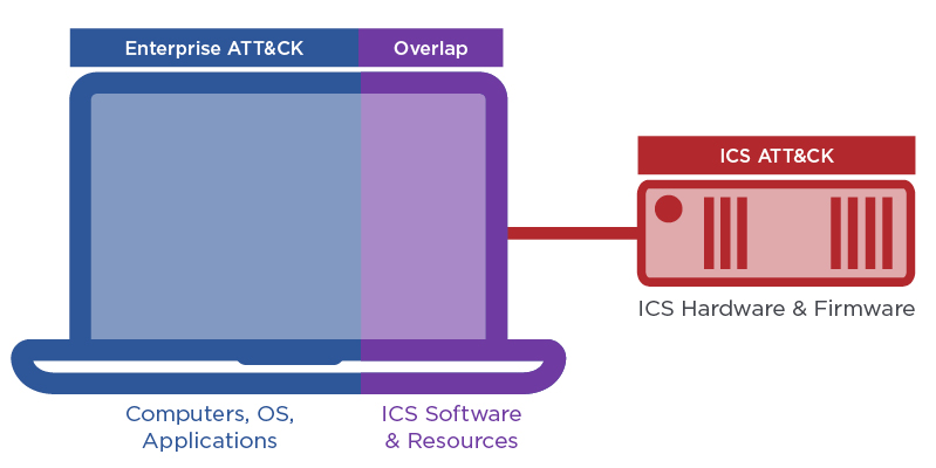
\includegraphics[width=0.9\textwidth]{img/attack-ICS.png}
    \caption{Endüstriyel Kontrol Sistemlerine (ICS) Yönelik Siber Saldırı Türleri}
    \label{fig:attack-ics}
\end{figure}

\subsection{ICS Taktikleri ve Teknikleri}

ATT\&CK for ICS, şu ana taktik kategorilerini içerir:

\begin{itemize}
\item \textbf{İlk Erişim (Initial Access):} Saldırganların ICS ağına ilk giriş yöntemleri.
\begin{itemize}
    \item Mühendislik İş İstasyonlarının Ele Geçirilmesi
    \item Dış Uzaktan Hizmetler
    \item İnternet Erişilebilir Cihaz
    \item Yeniden Satıcı/Tedarik Zinciri Ele Geçirme
\end{itemize}

\item \textbf{Keşif (Discovery):} ICS ortamını ve sistemlerini öğrenme teknikleri.
\begin{itemize}
    \item Kontrol Cihazı Keşfi
    \item I/O Modül Keşfi
    \item Seri Bağlantı Keşfi
    \item Program Organizasyon Birimi Keşfi
\end{itemize}

\item \textbf{Kalıcılık (Persistence):} Sistemde uzun süreli erişim sağlama yöntemleri.
\begin{itemize}
    \item Modül Firmware'i
    \item Sistem Firmware'i
    \item Proje Dosya Enfeksiyonu
\end{itemize}

\item \textbf{Yan Hareket (Lateral Movement):} ICS ağı içinde hareket etme teknikleri.
\begin{itemize}
    \item Programlama Yazılımı Kullanarak Erişim
    \item Uzak Hizmetler Üzerinden Hareket
    \item Veri Toplama Protokollerini Kötüye Kullanma
\end{itemize}

\item \textbf{Etki (Impact):} Sistemin işleyişini bozma veya kesintiye uğratma yöntemleri.
\begin{itemize}
    \item Kontrol Mantığının Değiştirilmesi
    \item Parametre Değişiklikleri
    \item Hizmet Kesintisi
    \item Güvenlik Enstrümantasyon Sisteminin Atlatılması
\end{itemize}
\end{itemize}

\subsection{ICS Savunma Stratejileri}

ATT\&CK for ICS çerçevesi, her teknik için karşı önlemler ve algılama yöntemleri önerir:

\begin{itemize}
\item \textbf{Ağ Segmentasyonu:} ICS ağının kurumsal ağdan ve internetten izole edilmesi.
\item \textbf{Erişim Kontrolü:} Sıkı erişim kontrol politikaları ve çok faktörlü kimlik doğrulama.
\item \textbf{Güvenlik İzleme:} ICS-spesifik anormallik tespiti ve olay izleme.
\item \textbf{Güvenlik Duvarları:} Endüstriyel protokolleri anlayan özelleştirilmiş güvenlik duvarları.
\item \textbf{Varlık Yönetimi:} Tüm ICS bileşenlerinin detaylı envanteri.
\end{itemize}

\subsection{Risk Değerlendirme ve Azaltma}

ICS güvenliği için risk değerlendirmesi, şu adımları içerir:

\begin{enumerate}
\item \textbf{Varlık Tanımlama:} Kritik ICS bileşenlerinin belirlenmesi.
\item \textbf{Tehdit Modelleme:} ATT\&CK for ICS kullanarak olası saldırı vektörlerinin belirlenmesi.
\item \textbf{Zafiyet Analizi:} Sistemdeki güvenlik açıklarının tespiti.
\item \textbf{Risk Değerlendirme:} Tehditlerin olasılık ve etki analizinin yapılması.
\item \textbf{Kontrol Seçimi:} Uygun güvenlik kontrollerinin belirlenmesi ve uygulanması.
\end{enumerate}

\section{Web Uygulama Güvenliği ve OWASP Framework}

Web uygulamaları, modern dijital ekosisteminde çok önemli bir role sahiptir ancak aynı zamanda siber saldırganların en çok hedeflediği varlıklar arasında yer alırlar. Web uygulama güvenliği, bu riskleri azaltmak ve kullanıcı verilerini korumak için hayati öneme sahiptir.

\subsection{OWASP Top 10 Zafiyetleri ve Azaltma Stratejileri}

Open Web Application Security Project (OWASP) Top 10, web uygulamalarındaki en kritik güvenlik risklerini listeleyen endüstri standardıdır. 2021 sürümü aşağıdaki tehditleri içermektedir:

\begin{enumerate}
\item \textbf{A01: Broken Access Control} - Erişim kontrolü zafiyetleri
\item \textbf{A02: Cryptographic Failures} - Kriptografik hatalar  
\item \textbf{A03: Injection} - Enjeksiyon saldırıları
\item \textbf{A04: Insecure Design} - Güvensiz tasarım
\item \textbf{A05: Security Misconfiguration} - Güvenlik yanlış yapılandırması
\item \textbf{A06: Vulnerable and Outdated Components} - Zafiyet bulunan bileşenler
\item \textbf{A07: Identification and Authentication Failures} - Kimlik doğrulama hataları
\item \textbf{A08: Software and Data Integrity Failures} - Yazılım ve veri bütünlüğü hataları
\item \textbf{A09: Security Logging and Monitoring Failures} - Güvenlik loglama ve izleme hataları
\item \textbf{A10: Server-Side Request Forgery (SSRF)} - Sunucu tarafı istek sahteciliği
\end{enumerate}

\subsection{Girdi Doğrulama, Çıktı Kodlama ve Parametreli Sorgular}

Güvenli web uygulama geliştirmenin temel prensipleri:

\begin{itemize}
\item \textbf{Girdi Doğrulama (Input Validation):} Tüm kullanıcı girdilerinin güvenilir olmadığı varsayılarak kapsamlı doğrulama yapılması
\item \textbf{Çıktı Kodlama (Output Encoding):} XSS saldırılarını önlemek için HTML, JavaScript ve CSS içeriğinin güvenli şekilde kodlanması
\item \textbf{Parametreli Sorgular (Parameterized Queries):} SQL enjeksiyonu saldırılarını önlemek için prepared statements kullanımı
\end{itemize}

\subsection{Kimlik Doğrulama ve Oturum Yönetimi Güvenliği}

Güvenli kimlik doğrulama ve oturum yönetimi için:

\begin{itemize}
\item Güçlü parola politikaları ve çok faktörlü kimlik doğrulama
\item Güvenli oturum token'ları ve uygun timeout değerleri
\item Session fixation ve session hijacking saldırılarına karşı koruma
\end{itemize}

\subsection{Cross-Site Scripting (XSS) ve Cross-Site Request Forgery (CSRF)}

\begin{itemize}
\item \textbf{XSS Koruması:} Content Security Policy (CSP), girdi doğrulama ve çıktı kodlama
\item \textbf{CSRF Koruması:} CSRF token'ları, SameSite cookie attribute kullanımı
\end{itemize}

\subsection{Content Security Policy (CSP) ve Güvenlik Header'ları}

Modern web uygulamalarında kullanılması gereken güvenlik header'ları:

\begin{itemize}
\item Content-Security-Policy
\item X-Frame-Options  
\item X-Content-Type-Options
\item Strict-Transport-Security
\item Referrer-Policy
\end{itemize}

\section{API Güvenliği ve Microservices Mimarisi}

API güvenliği, modern dağıtık sistemlerde kritik öneme sahiptir. Microservices mimarilerinin yaygınlaşmasıyla API güvenliği daha da kritik hale gelmiştir.

\subsection{RESTful API Güvenliği En İyi Uygulamaları}

\begin{itemize}
\item HTTPS kullanımı zorunluluğu
\item Uygun HTTP metod kullanımı
\item Rate limiting ve throttling
\item API versiyonlama güvenliği
\item Error handling ve bilgi sızıntısı önleme
\end{itemize}

\subsection{OAuth 2.0, OpenID Connect ve JWT Token Güvenliği}

Modern API kimlik doğrulama ve yetkilendirme standartları:

\begin{itemize}
\item OAuth 2.0 akışları ve güvenlik hususları
\item OpenID Connect identity layer implementasyonu
\item JWT token güvenliği: imzalama, şifreleme ve doğrulama
\item Token lifecycle yönetimi
\end{itemize}

\subsection{API Gateway Güvenlik Özellikleri ve Rate Limiting}

API Gateway'lerin güvenlik rolleri:

\begin{itemize}
\item Merkezi kimlik doğrulama ve yetkilendirme
\item Rate limiting ve DDoS koruması
\item Request/response transformation
\item API monitoring ve analytics
\end{itemize}

\subsection{GraphQL Güvenlik Hususları}

GraphQL'in getirdiği yeni güvenlik zorlukları:

\begin{itemize}
\item Query depth limiting
\item Query complexity analysis
\item Introspection devre dışı bırakma
\item Field-level authorization
\end{itemize}

\subsection{Microservices İletişim Güvenliği (mTLS, Service Mesh)}

Microservices arası güvenli iletişim:

\begin{itemize}
\item Mutual TLS (mTLS) implementasyonu
\item Service mesh güvenlik özellikleri (Istio, Linkerd)
\item Zero trust network principles
\item Service-to-service authentication
\end{itemize}

\section{Mobil Uygulama Güvenliği}

Mobil uygulama güvenliği, kullanıcı verilerini korumak ve yetkisiz erişimi önlemek için kritik öneme sahiptir. Mobil uygulamalar, hem cihazda hem de sunucu tarafında çeşitli güvenlik riskleriyle karşı karşıyadır. Bu riskler, veri sızıntıları, kötü amaçlı yazılım bulaşmaları ve kimlik avı saldırılarını içerir.

\subsection{iOS Uygulama Güvenliği: Kod İmzalaması, App Transport Security (ATS)}

\begin{itemize}
\item \textbf{Kod İmzalaması (Code Signing):} Bir iOS uygulamasının, Apple tarafından yetkilendirilmiş bir geliştirici tarafından imzalandığını doğrular. Bu imza, uygulamanın dağıtıldıktan sonra kurcalanmadığını ve değiştirilmediğini garanti eder.
\item \textbf{App Transport Security (ATS):} iOS 9 ve sonraki sürümler için varsayılan olarak etkin olan bir güvenlik özelliğidir. ATS, bir uygulamanın sunucuyla kurduğu tüm ağ bağlantılarının, minimum güvenlik gereksinimlerini (örn. TLS 1.2 veya daha yeni bir sürüm, güçlü anahtar boyutları) karşılayan güvenli bir TLS protokolüyle şifrelenmesini zorunlu kılar.
\end{itemize}
\subsection{Android Uygulama Güvenliği: ProGuard, Sertifika Sabitleme (Certificate Pinning)}
\begin{itemize}
\item \textbf{ProGuard:} Kod gizleme (obfuscation) ve optimizasyon aracıdır. Uygulamanın kodunu okunması ve tersine mühendislikle analiz edilmesi zor bir hale getirerek, fikri mülkiyetin korunmasına yardımcı olur. \texttt{build.gradle} dosyasında kolayca etkinleştirilebilir.
\item \textbf{Sertifika Sabitleme (Certificate Pinning):} Bir uygulamanın yalnızca belirli, önceden tanımlanmış sunucu sertifikalarına veya ortak anahtarlara güvenmesini sağlayan bir tekniktir. Bu, ortadaki adam (MITM) saldırılarına karşı güçlü bir savunma mekanizmasıdır. Ancak bu teknik, sunucu tarafındaki sertifika rotasyonu gibi durumlar için alternatif sabitleme (\texttt{pinset}) mekanizmalarıyla dikkatli bir şekilde yönetilmelidir.
\end{itemize}

\subsection{Mobil Uygulama Sızma Testi Metodolojileri}

Mobil uygulama sızma testi, uygulamadaki zafiyetleri bulmak için gerçek dünya saldırılarını simüle eder.

\begin{itemize}
\item \textbf{Statik Analiz:} Uygulama çalıştırılmadan kaynak kodu veya ikili dosyaları incelenir. Bu yöntem, sabit kodlanmış kimlik bilgileri ve güvensiz kodlama pratikleri gibi sorunları tespit eder.
\item \textbf{Dinamik Analiz:} Uygulama çalışırken, ağ trafiği, bellek kullanımı ve çalışma zamanı davranışı izlenir. Bu, çalışma zamanı zafiyetlerini (örn. güvensiz veri depolama, zafiyetli iletişim) ortaya çıkarır.
\item \textbf{En İyi Uygulamalar:} Mobil uygulama sızma testleri, OWASP Mobile Application Security Testing Guide (MASTG) gibi çerçeveler kullanılarak sistematik bir şekilde yürütülmelidir.
\end{itemize}
\subsection{Binary Koruma ve Anti-tampering Teknikleri}
\begin{itemize}
\item \textbf{İkili Koruma (Binary Protection):} Uygulama ikililerini tersine mühendislikten ve izinsiz değişikliklerden korumayı amaçlar.
\item \textbf{Anti-tampering:} Uygulamanın çalışırken veya statik haldeyken kurcalanmasını (değiştirilmesini) engellemek için tasarlanmış tekniklerdir.
\item \textbf{Teknikler:} Kod gizleme (obfuscation), dosya bütünlüğü kontrolü, hata ayıklama (debugger) algılama, jailbreak/root algılama gibi çeşitli yöntemler kullanılır.
\item \textbf{Savunma:} Statik (obfuscation, encryption) ve dinamik (RASP) önlemleri birleştiren çok katmanlı bir yaklaşım benimsenmelidir. RASP, çalışma zamanında kurcalama girişimlerini algılayıp yanıt vererek dinamik saldırılara karşı koruma sağlar.
\end{itemize}

\section{Web3 ve Blockchain Güvenliği}

Blockchain teknolojisi ve Web3 ekosistemin güvenliği, merkezi olmayan uygulamaların güvenli işlemesini sağlamak için kritik öneme sahiptir. Bu teknolojiler hem yenilikçi güvenlik özellikleri sunar hem de geleneksel güvenlik modellerinin ötesinde yeni zorluklar yaratır.

\subsection{Merkezi Olmayan Uygulamalar (DApps) Güvenliği}

Blockchain tabanlı uygulamaların güvenlik zorlukları ve korunma yöntemleri, geleneksel web uygulamalarından köklü farklılıklar gösterir. DApps, immutable (değiştirilemez) kod yapısı nedeniyle güvenlik açıklarının düzeltilmesini zorlaştırır.

\textbf{DApp Güvenlik Bileşenleri:}
\begin{itemize}
    \item \textbf{Smart Contract Layer:} İş mantığının çalıştığı katman
    \item \textbf{Frontend Interface:} Kullanıcı etkileşim katmanı  
    \item \textbf{Blockchain Network:} Altyapı ve consensus katmanı
    \item \textbf{Wallet Integration:} Kimlik doğrulama ve işlem imzalama
\end{itemize}

\textbf{Common DApp Security Risks:}
\begin{lstlisting}[breaklines=true,basicstyle=\ttfamily\footnotesize]
// Reentrancy saldırısından korunma örneği
pragma solidity ^0.8.0;

contract SecureDApp {
    mapping(address => uint256) private balances;
    bool private locked;
    
    modifier noReentrancy() {
        require(!locked, "Reentrant call");
        locked = true;
        _;
        locked = false;
    }
    
    function withdraw(uint256 amount) external noReentrancy {
        require(balances[msg.sender] >= amount, "Insufficient balance");
        
        // Checks-Effects-Interactions pattern
        balances[msg.sender] -= amount; // Effect önce
        
        (bool success, ) = msg.sender.call{value: amount}(""); // Interaction sonra
        require(success, "Transfer failed");
    }
}
\end{lstlisting}

\subsection{Smart Contract Güvenliği}

Akıllı sözleşmelerde karşılaşılan güvenlik açıkları ve audit süreçleri, blockchain ekosistemin güvenliğinin temelini oluşturur. Smart contract'lar immutable oldukları için güvenlik testleri dağıtımdan önce kritik önem taşır.

\textbf{Smart Contract Security Audit Process:}
\begin{enumerate}
    \item \textbf{Static Code Analysis:} Otomatik güvenlik tarama araçları (Slither, Mythril)
    \item \textbf{Manual Security Review:} Deneyimli auditörler tarafından kod incelemesi
    \item \textbf{Formal Verification:} Matematiksel doğrulama yöntemleri
    \item \textbf{Dynamic Testing:} Test ağlarında gerçek senaryo simülasyonları
\end{enumerate}

\textbf{Critical Smart Contract Vulnerabilities:}
\begin{itemize}
    \item \textbf{Reentrancy Attacks:} Fonksiyonun tamamlanmadan tekrar çağrılması
    \item \textbf{Integer Overflow/Underflow:} Sayısal taşma güvenlik açıkları
    \item \textbf{Access Control Issues:} Yetkilendirme kontrollerinin eksikliği
    \item \textbf{Front-running:} İşlem sıralamasını manipüle etme saldırıları
    \item \textbf{Flash Loan Attacks:} Anında borç mekanizmalarının kötüye kullanımı
\end{itemize}

\subsection{DeFi ve NFT Güvenlik Riskleri}

Merkezi olmayan finans (DeFi) ve NFT'lerdeki güvenlik sorunları, milyarlarca dolarlık varlığın risk altında olmasına neden olmaktadır.

\textbf{DeFi Security Architecture:}
\begin{lstlisting}[breaklines=true,basicstyle=\ttfamily\footnotesize]
// DeFi protocol güvenlik örneği
contract SecureDeFiProtocol {
    using SafeMath for uint256;
    
    // Price oracle manipulation koruması
    IPriceOracle[] public priceOracles;
    uint256 public constant ORACLE_DEVIATION_THRESHOLD = 5; // %5
    
    function getSecurePrice(address token) public view returns (uint256) {
        uint256[] memory prices = new uint256[](priceOracles.length);
        
        for (uint i = 0; i < priceOracles.length; i++) {
            prices[i] = priceOracles[i].getPrice(token);
        }
        
        // Median price calculation ve outlier detection
        uint256 medianPrice = calculateMedian(prices);
        validatePriceDeviation(prices, medianPrice);
        
        return medianPrice;
    }
    
    function validatePriceDeviation(uint256[] memory prices, uint256 median) 
        internal pure {
        for (uint i = 0; i < prices.length; i++) {
            uint256 deviation = prices[i] > median ? 
                prices[i].sub(median) : median.sub(prices[i]);
            uint256 deviationPercent = deviation.mul(100).div(median);
            
            require(deviationPercent <= ORACLE_DEVIATION_THRESHOLD, 
                    "Price oracle deviation too high");
        }
    }
}
\end{lstlisting}

\textbf{NFT Security Considerations:}
\begin{itemize}
    \item \textbf{Metadata Immutability:} NFT metadatalarının değiştirilemezliği
    \item \textbf{Royalty Bypass:} Telif hakkı ödemelerinin atlanması
    \item \textbf{Wash Trading:} Yapay fiyat manipülasyonu
    \item \textbf{Counterfeit NFTs:} Sahte NFT üretimi ve satışı
\end{itemize}

\subsection{Mobil Backend API Güvenliği Hususları}

Mobil uygulamalar, kullanıcı verilerini yönetmek ve iş mantığını yürütmek için arka uç API'leriyle iletişim kurar. Bu API'lerin güvenliği, en az mobil uygulama kadar kritik öneme sahiptir. Mobil backend API güvenliği, bu raporun Bölüm 4.3'te ele alınan genel API güvenliği ilkelerine dayanır. Bu, hem platformlar arası güvenlik tutarlılığını hem de savunmada derinlik prensibini pekiştirir. API'ler için TLS şifrelemesi, güçlü kimlik doğrulama, hız sınırlama ve API ağ geçidi kullanımı gibi uygulamalar, mobil ekosistemin bütünlüğünü korumada anahtar rol oynar.
